\chapter{Event categorisation}
\label{chap:categorisation}

\section{Introduction}
\label{cat:sec:intro}

The basic experimental method for the observation of the \Hgg decay is to search for a resonance in the continuous \SM diphoton invariant mass spectrum. The sensitivity of this method is enhanced by the categorisation of events by their expected mass resolution. Furthermore, additional particles in the final state can be explointed to gain information about the process by which the Higgs boson was produced in each event. This allows the measurement of the cross-section of each production mode individually. This information can be used to probe the strength of the Higgs boson's interaction with the individual particles involved in each mode. %These considerations motivate the following categorisation scheme. 

To first order, the most common production mode, \ggH, produces a Higgs boson in isolation. This leaves only the photons resulting from \Hgg decay in the final state. The other production modes (\VBF, \VH and \ttH) produce the Higgs boson with additional particles. The \VBF mode has two quarks in the final state, which subsequently hadronize to form jets. The \VH mode produces a Higgs boson in association with a \PW or \PZ boson, which subsequently decays to charged leptons, neutrinos or quarks, leading to reconstructed leptons, \MET and jets. Finally, the \ttH mode produces the Higgs boson in association with two top quarks, which decay to bottom quarks and either hadrons or leptons. These distinctive topologies can be used to categorise events. The categorisation benefits from information about the expected mass resolution of the diphoton, which is obtained with the \BDT described in \Sec~\ref{cat:sec:dipho_bdt}. The categories targeting \VBF, \VH and \ttH events are then discussed in \Sec\s~\ref{cat:sec:vbftag},~\ref{cat:sec:vhtag} and~\ref{cat:sec:tthtag}. Finally, the inclusive \Untagged categories and the categorisation hierarchy are discussed in \Sec\s~\ref{cat:sec:untagged} and~\ref{cat:sec:hierarchy}.

\section{Diphoton BDT}
\label{cat:sec:dipho_bdt}

The ranking of events by their expect mass resolution or signal-to-background ratio is obtained using a per-diphoton \BDT, which is hereafter referred to as \DiPhoBdt. The objectives of the \DiPhoBdt are to separate signal-like diphotons (produced by the decay of a Higgs boson) from the \SM background diphotons, and to assign a high output score to diphotons with a good mass resolution and where both individual photons have high \PhoIdBdt scores. 

Diphotons are composed of pairs of photons and a primary vertex (selected as described in Chapter~\ref{chap:reconstruction}). Before the \DiPhoBdt is applied, the diphotons are required to satisfy the following requirements: both photons must pass a loose requirement on their \PhoIdBdt score, and the \pT of the leading (subleading) photon must be above $\mgg/3$ ($\mgg/4$).

The \DiPhoBdt is required to assess diphotons independently of their invariant mass, otherwise the \mH value of the training sample would introduce a bias in the output score. The input variables for the \DiPhoBdt are therefore chosen to be uncorrelated with the invariant mass of the diphoton system:

\begin{itemize}
\item the transverse momentum of each photon, divided by $\mgg$ to remove the correlation with \mH;
\item the $\eta$-position of each photon;
\item the \PhoIdBdt output score of each photon;
\item $\cos(\Delta\phi)$, the cosine of the angle between the photons in the $\phi$-direction;
\item \sigmarv, the per-event estimated mass resolution of the diphoton, assuming that the selected vertex is within 1\cm of the true vertex in the $z$-direction ($\Delta z \leq 1\cm$);
\item \sigmawv, the per-event estimated mass resolution of the diphoton, assuming that the selected vertex is more than 1\cm away from the true vertex in the $z$-direction ($\Delta z > 1\cm$);
\item $p_{rv}$, the per-event estimate of the probability that the correct vertex was chosen, obtained using the \VtxProbBdt described in \Sec~\ref{reco:sec:vtx_prob}.
\end{itemize}

The per-event estimated mass resolutions are calculated from the individual photon energy resolution estimates, labelled $\sigma^E_{\gamma_1}/E_{\gamma_1}$ and $\sigma^E_{\gamma_2}/E_{\gamma_2}$, obtained from the semiparametric regression \PhoEnergyBdt described in \Sec~\ref{sec:reco:photon:phoenergybdt}. If $\Delta z \leq 1\cm$, the dominant contributions to the uncertainty on the mass resolution are the energy resolutions of each photon. Assuming Gaussian resolution functions, \sigmarv can be obtained by simply adding the individual relative photon energy resolutions in quadrature:
\begin{equation}
\sigmarv= \frac{1}{2} \sqrt{({\sigma^E_{\gamma_1}}/{E_{\gamma_1}})^2 +({\sigma^E_{\gamma_2}}/{E_{\gamma_2}})^2 }.
\end{equation} 
However, if $\Delta z > 1\cm$, the uncertainty on the opening angle contributes significantly to the mass resolution. The effect is modelled by including an additional term which represents the uncertainty on the mass due to the uncertainty on the vertex position, labelled $\sigma^V_{\gamma\gamma}$. The distance between the true vertex and the selected vertex follows a Gaussian distribution which has a width equal to the width of the beamspot multiplied by $\sqrt{2}$. Given the spatial positions of the photons, $\sigma^V_{\gamma\gamma}$ can therefore be calculated explicitly, and included in the sum in quadrature:
\begin{equation}
\sigmawv= \sqrt{(\sigmarv)^2 +(\sigma^V_{\gamma\gamma}/\mgg)^2 }.
\end{equation} 

The \DiPhoBdt is trained on simulated sampled of signal and background processes. For the signal samples, events from different productions modes (all $\mH=125\GeV$) are mixed according to their cross-section. The signal events used for training are also re-weighted by a factor $w$ given by: 
\begin{equation}
w= \frac{p_{rv}}{\sigmarv}+\frac{1-p_{rv}}{\sigmawv},
\end{equation} 
which codifies the fact that the signal-to-background ratio is inversely proportional to the mass resolution. This step ensures that the \DiPhoBdt gives a high score to events with good mass resolution.
The background for the training is composed of simulated diphotons originating from the irreducible and reducible \SM background processes. 

\Fig~\ref{fig:cat:diphobdt_a} shows the \DiPhoBdt output score for signal and background events in the range $100\GeV < \mgg < 180\GeV$, where a transformation is applied to flatten the signal distribution, so that the efficiency of a particular selection can be easily read. The \DiPhoBdt output score is validated using \Zee events in data and simulation, as can be seen on \Fig~\ref{fig:cat:diphobdt_b}.
\begin{figure}[h]
\centering
 \subfloat[]{
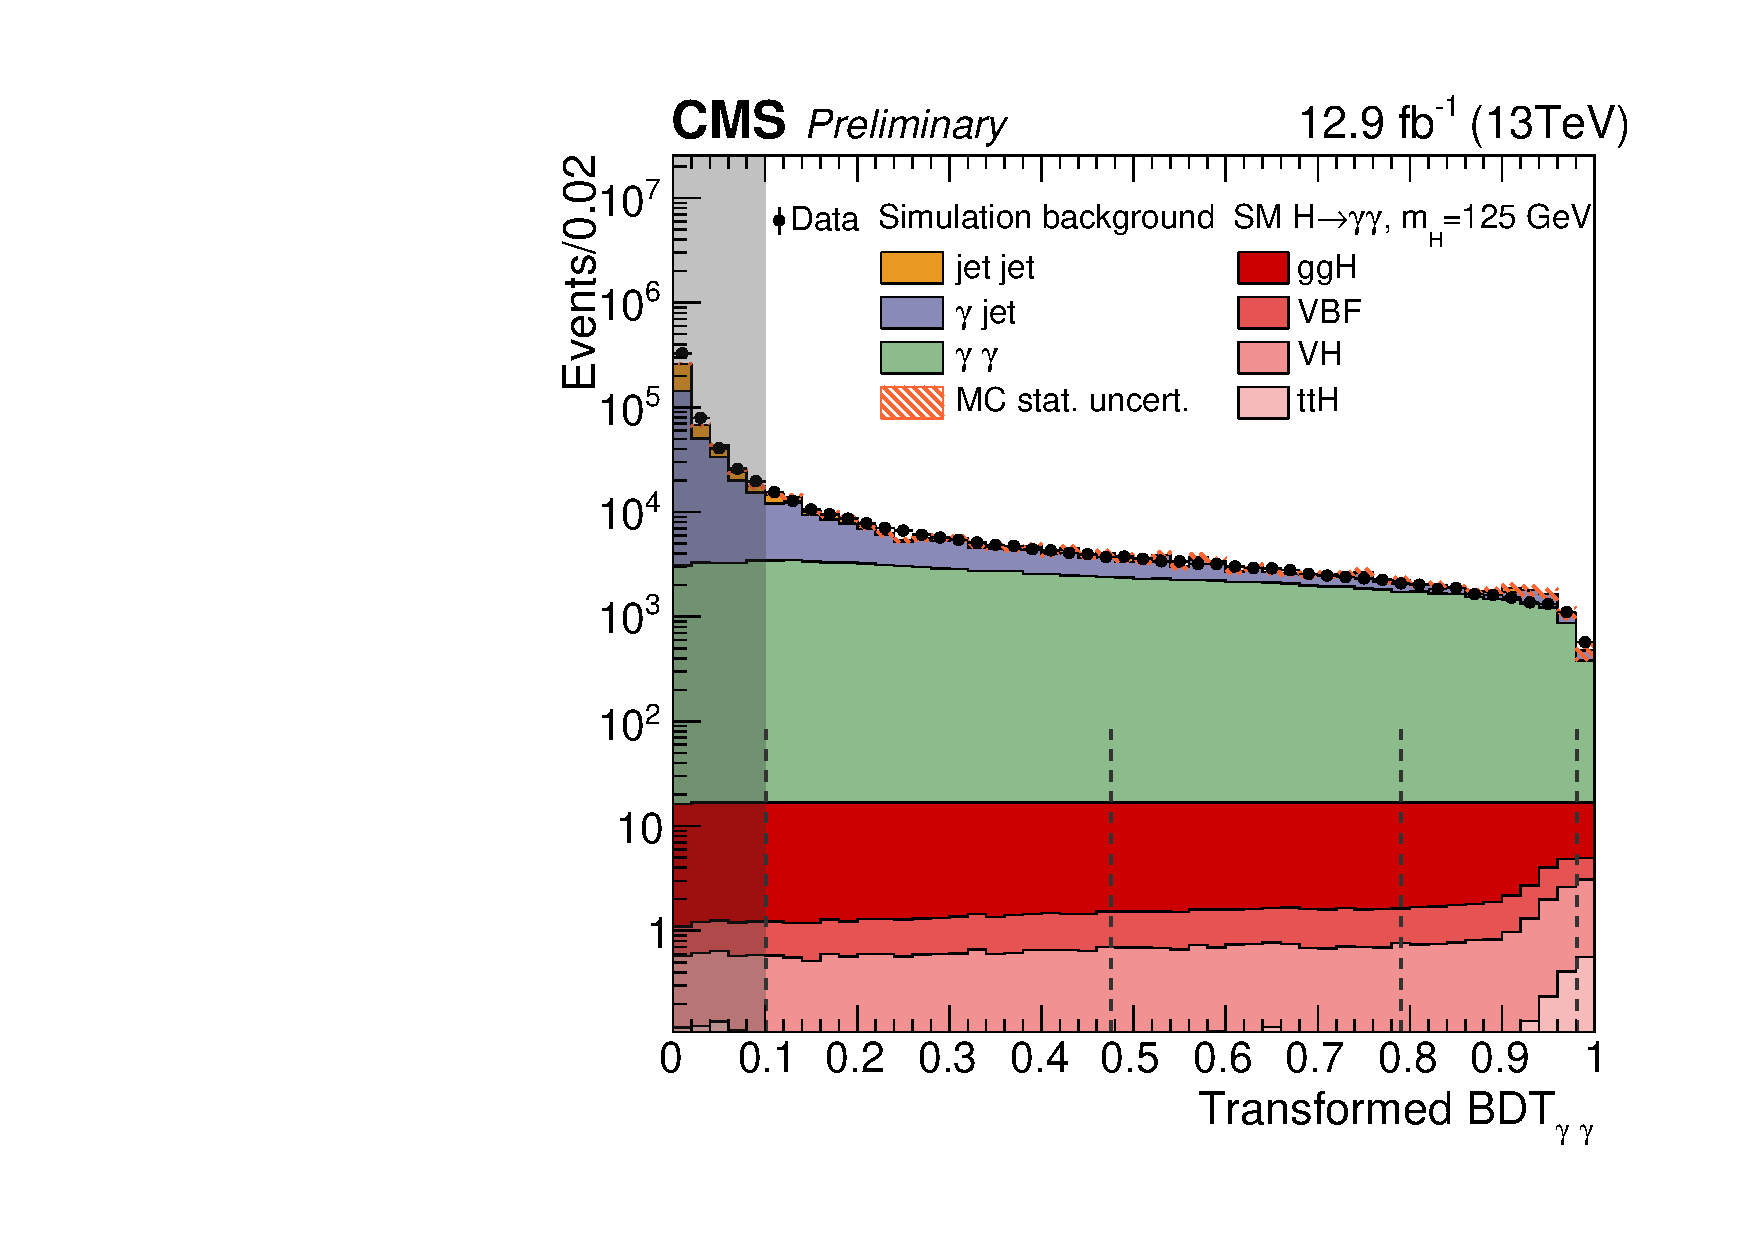
\includegraphics[width=0.5\textwidth]{catFigures/stack_scaled_resultFlat_mc_cat0_noratio.pdf}
\label{fig:cat:diphobdt_a}
}
 \subfloat[]{
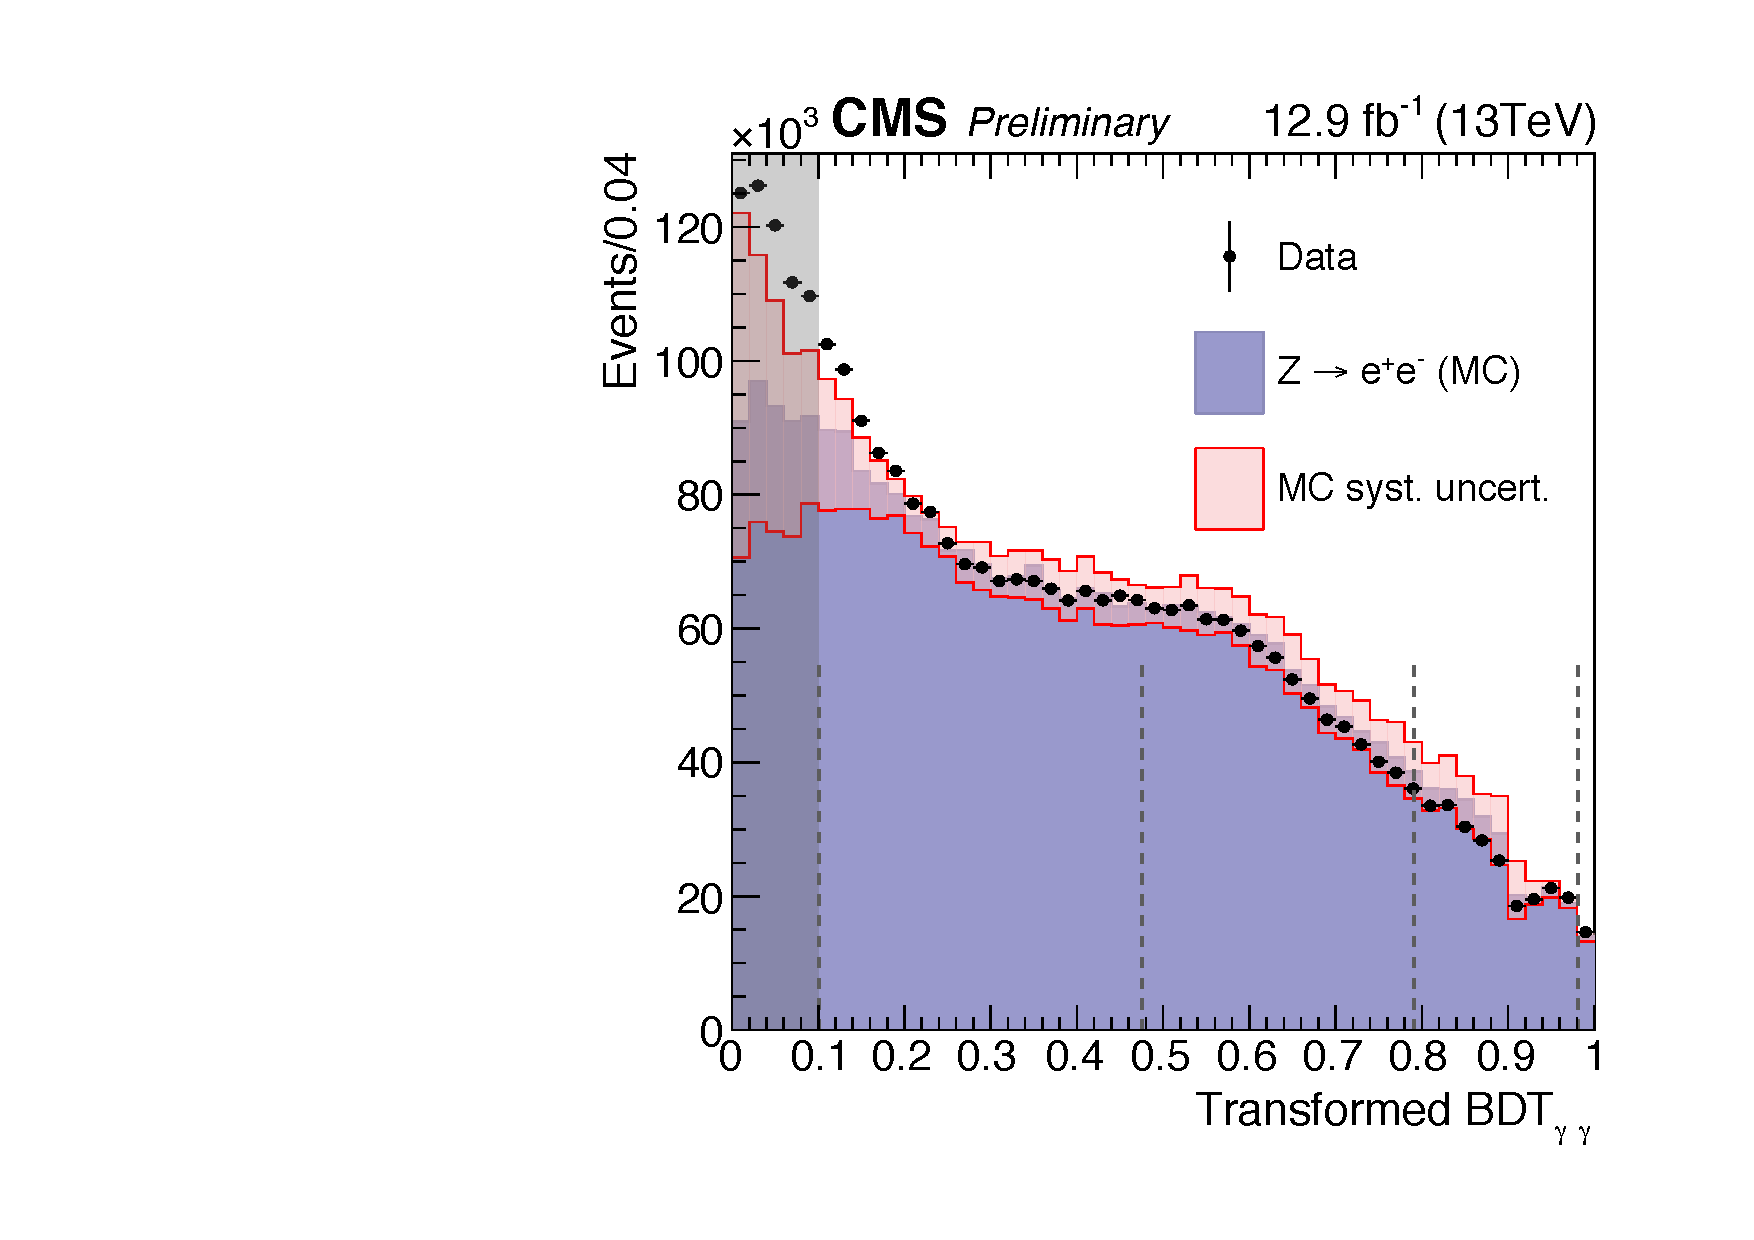
\includegraphics[width=0.50\textwidth]{catFigures/BDTTransfSyst_TrasfBDT_lin_1sigma_shiftPlusTransf_new_noratio.pdf}
\label{fig:cat:diphobdt_b}
}
\caption{ (a) The transformed \DiPhoBdt score for simulated signal and background events in the range $100\GeV < \mgg < 180\GeV$. The transformation flattens the signal distribution. (b) The transformed \DiPhoBdt score for \Zee events in data and simulation, where the electrons are reconstructed as photons. The pink shading represents the systematic uncertainty associated with the \PhoIdBdt and the \PhoEnergyBdt. For both (a) and (b), the vertical dashed lines represent the boundaries of the Untagged categories described in \Sec~\ref{cat:sec:untagged}, while the grey shading represents the area for which diphotons are rejected.}
\label{fig:cat:diphobdt}
\end{figure}

\section{\VBFTag categories }
\label{cat:sec:vbftag}

%Higgs bosons in \CMS are produced chiefly via the \ggH production mode in the LHC environment. In this mode, the final state of the interaction involving the Higgs boson contains only the Higgs boson decay products to first order. Other production modes, by contrast, produce a Higgs boson in association with other particles. The additional particles can therefore be used to identify Higgs bososn events produced via \VBF, \VH or \ttH. 
The \VBF production mode has a cross-section approximately ten times smaller than that of the \ggH mode. However, it produces the Higgs boson in association with two quarks, which result in two high-\pT jets when reconstructed. This distinctive topology allows the identification of \VBF events. For this reason, although \VBF events occur much less frequently than \ggH events, the most sensitive \VBFTag category has a signal-to-background ratio comparable to the most sensitive category in the analysis (the \Untagged 0 category). Defining \VBFTag categories therefore significantly improves the overall sensitivity of the analysis.

The \VBFTag categories are obtained by selecting events which contain two high-\pT jets. For each diphoton candidate, the individual jets are obtained as described in \Sec~\ref{reco:sec:jets} after \PFCHS with respect to the selected vertex. Candidate \VBFTag events are required to have at least two jets which pass the \PU removal requirements and are separated from \PF photon candidates by $\Delta R > 0.5$. The leading (subleading) jet, i.e~the one with the highest (second-highest) \pT in the event, is required to satisfy $\pT > 30 \GeV$ ($\pT > 20 \GeV$). For events passing these requirements, an additional selection on the invariant mass of the \emph{dijet} composed of the leading and subleading jets, \mjj, is imposed: $\mjj > 250\GeV$. %Events which satistfy all of the above are said to pass the \emph{dijet preselection}.

For events passing the dijet preselection described above, the \VBFTag categorisation proceeds as follows. First, a per-event \BDT, which is hereafter referred to as \DiJetBdt, is used to identify \VBF-like dijets. %The \DiJetBdt is trained to treat simulated \VBF events as signal, and to treat simulated \ggH events (where dijets are formed from \PU and initial or final state radiation) and \SM processes which produce jets as background. 
The \DiJetBdt does not have any knowledge of the quality and mass resolution of the diphoton, so a further per-event \BDT, referred to as the \DiPhoDiJetBdt, is used to recover this information. The \DiPhoDiJetBdt has the \DiPhoBdt and the \DiJetBdt output scores among its inputs variables. It is thus able to combine the \VBF-like dijet identification power of one \BDT with with mass resolution information from the other. %In the \DiPhoDiJetBdt, \ggH events cannot be treated as background since the \DiPhoBdt would not be well-behaved. So \ggH events are treated as neither signal nor background when training the \DiPhoDiJetBdt. 
A selection on the output score of the \DiPhoDiJetBdt is then used to choose events for the \VBFTag categories.

The \DiJetBdt is designed to use the kinematic properties of the diphoton-dijet system to identify \VBF-like events where the Higgs boson decayed via \Hgg. It is trained on simulated samples of diphoton events where the signal is defined as \VBF (\Hgg) events and the background consists of samples of \SM events with a diphoton and a dijet in the final state, in addition to a simulated sample of \ggH events where dijets are formed from \PU and initial or final state radiation. The input variables for this \BDT are listed below:
\begin{itemize}
\item the invariant-mass-scaled transverse momentum ($\pT/\mgg$) for the leading and subleading photons in the diphoton candidate;
\item $\pt^{\text{j}_1}$ and $\pt^{\text{j}_2}$, the transverse momenta of the leading and subleading jets in the dijet;
\item \mjj;
\item $|\eta_{\text{j}_1} - \eta_{\text{j}_2}|$, the separation of the jets in the dijet in the $\eta$-direction;
\item $\eta^{*} = \eta_{\gamma_1+\gamma_2} - (\eta_{j_1}+\eta_{j_2})/2$, the \emph{Zeppenfeld} variable~\cite{Zeppenfeld} where $\eta_{\gamma_1+\gamma_2}$ refers to the $\eta$-position of the vector sum of the photon momenta;
\item $|\phi_{\gamma\gamma} - \phi_\text{jj}|$, the separation of the dijet and the diphoton in the $\phi$-direction.
\end{itemize}

The distributions of the \DiJetBdt output scores for each simulated signal sample are shown in \Fig~\ref{fig:cat:dijetbdt_sig}. The distributions of the \DiJetBdt output scores for data and simulated background samples (and some simulated signal samples) are shown in \Fig~\ref{fig:cat:dijetbdt_all}. 

\begin{figure}[h]
\centering
 \subfloat[\DiJetBdt output by production mode]{
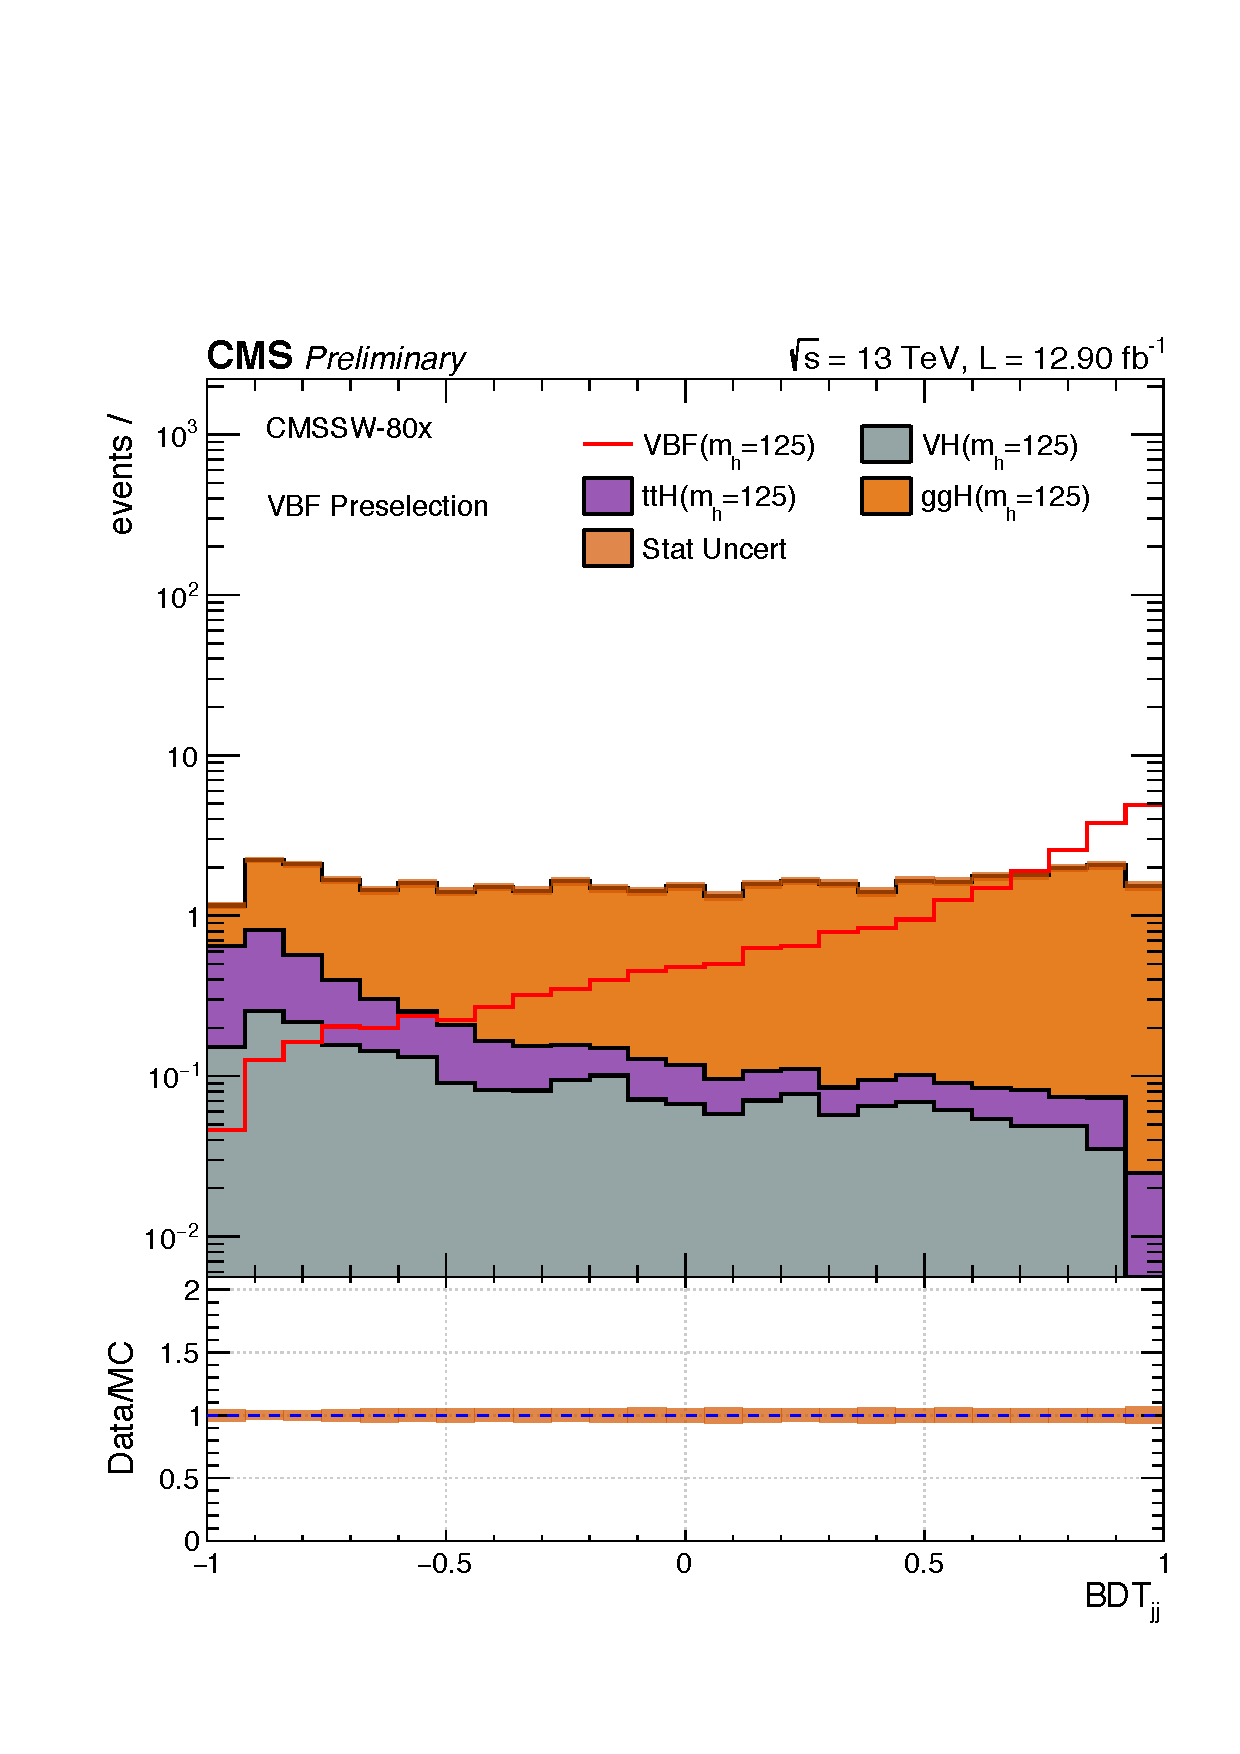
\includegraphics[width=0.45\textwidth]{catFigures/stack_histogram_dijet_mva_signal_14-07-2016_.pdf}
\label{fig:cat:dijetbdt_sig}
}
 \subfloat[\DiJetBdt output comparing data and simulated signal and background]{
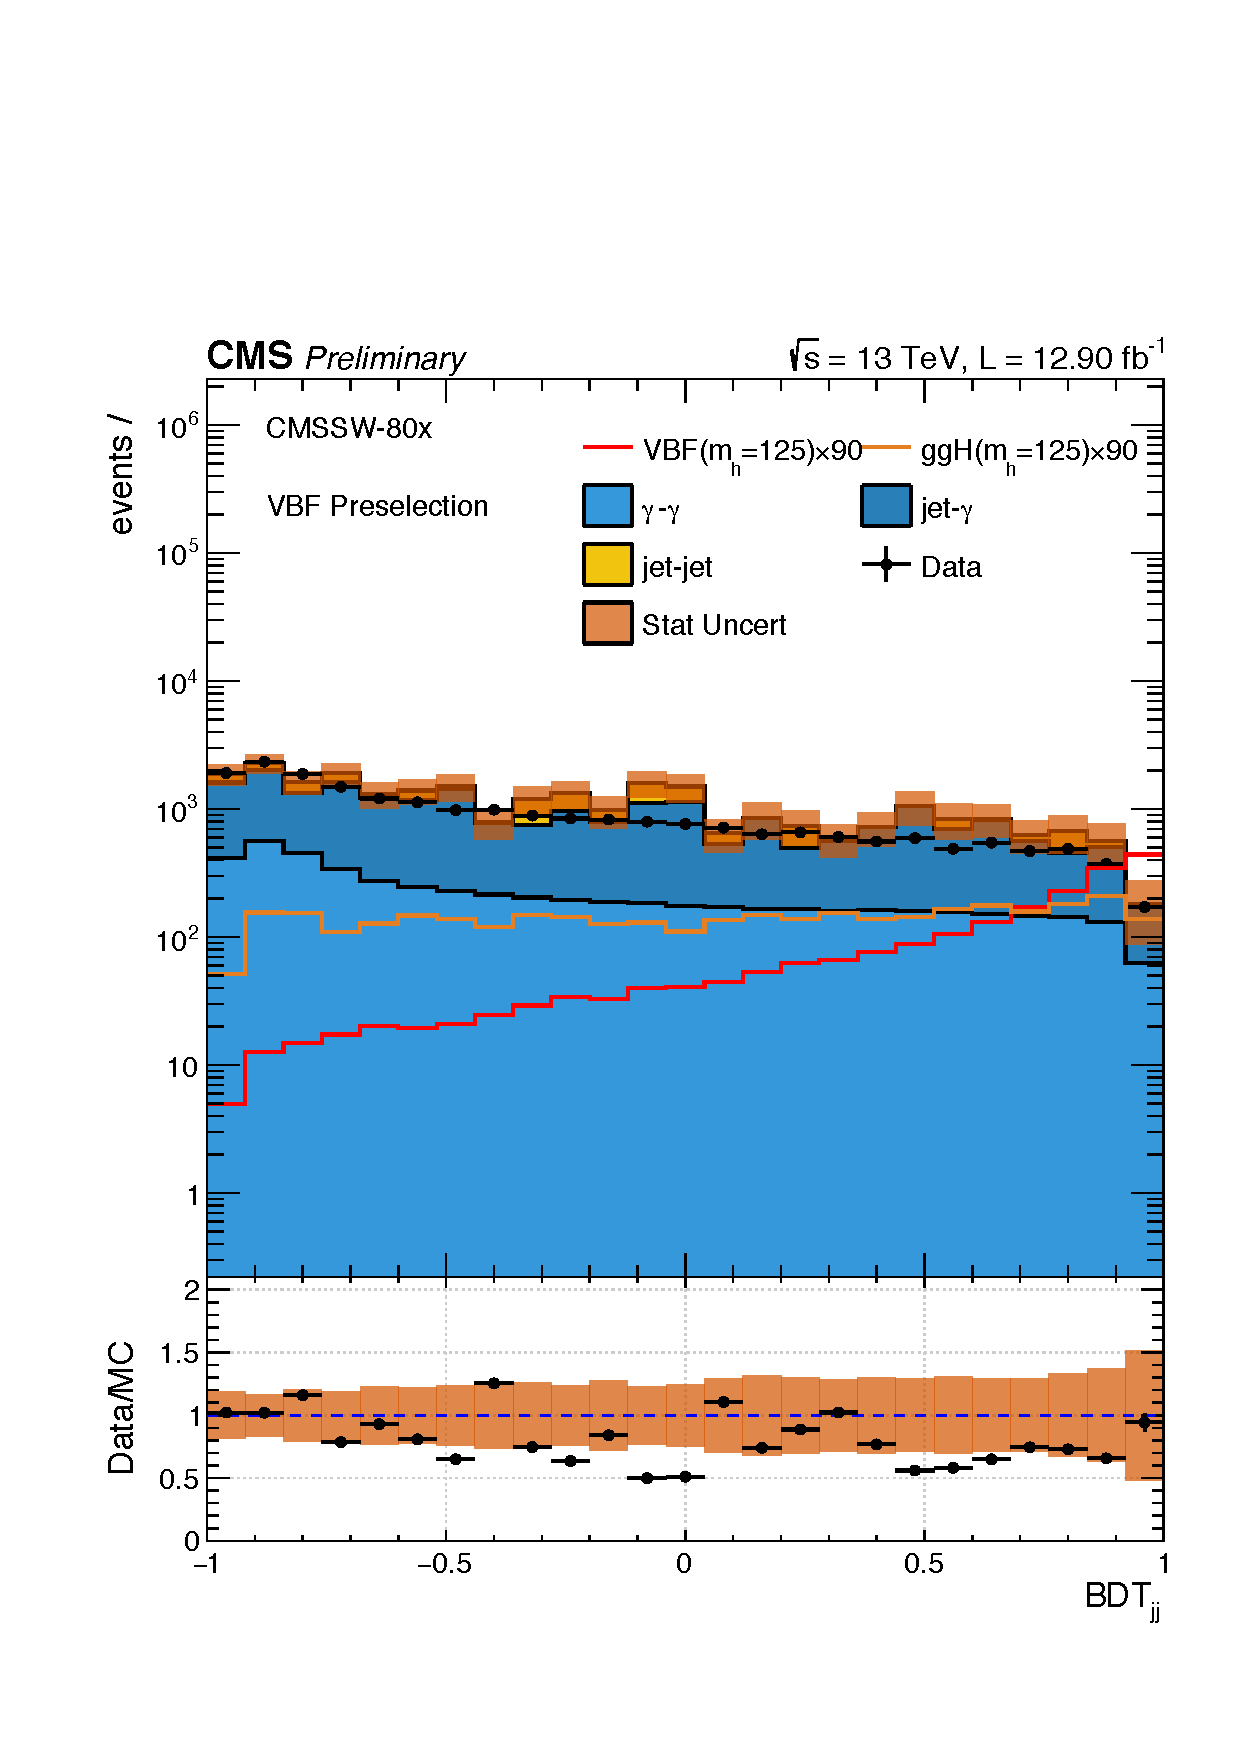
\includegraphics[width=0.45\textwidth]{catFigures/stack_histogram_dijet_mva_VBF_14-07-2016_.pdf}
\label{fig:cat:dijetbdt_all}
}
\caption{The output scores of the \DiJetBdt split by simulated production mode and comparing data and simulated signal and background.}
\label{fig:cat:dijet_bdt}
\end{figure}

The \DiPhoDiJetBdt is designed to re-introduce information about the sensitivity of signal events while maintaining the power to identify \VBF-like events. This is obtained by training the \BDT on simulated events where the signal is a sample of \VBF \Hgg events, while the background is composed of the \SM diphoton background samples, as for the \DiJetBdt training. In this case, \ggH events are treated as neither signal nor background. The inputs to the \BDT are the following:
\begin{itemize}
\item the output score of the \DiPhoBdt;
\item the output score of the \DiJetBdt;
\item $\pT^{\gamma\gamma}/\mgg$, the invariant-mass-scaled momentum of the diphoton system, which is included since it has a significant correlation to both the other inputs.
\end{itemize}

The distributions of the \DiPhoDiJetBdt output scores for each simulated signal sample are shown in \Fig~\ref{fig:cat:diphodijetbdt_sig}. The distributions of the \DiJetBdt output scores for data and simulated background samples (and some simulated signal samples) are shown in \Fig~\ref{fig:cat:diphodijetbdt_all}. 

\begin{figure}[h]
\centering
 \subfloat[\DiPhoDiJetBdt output by production mode]{
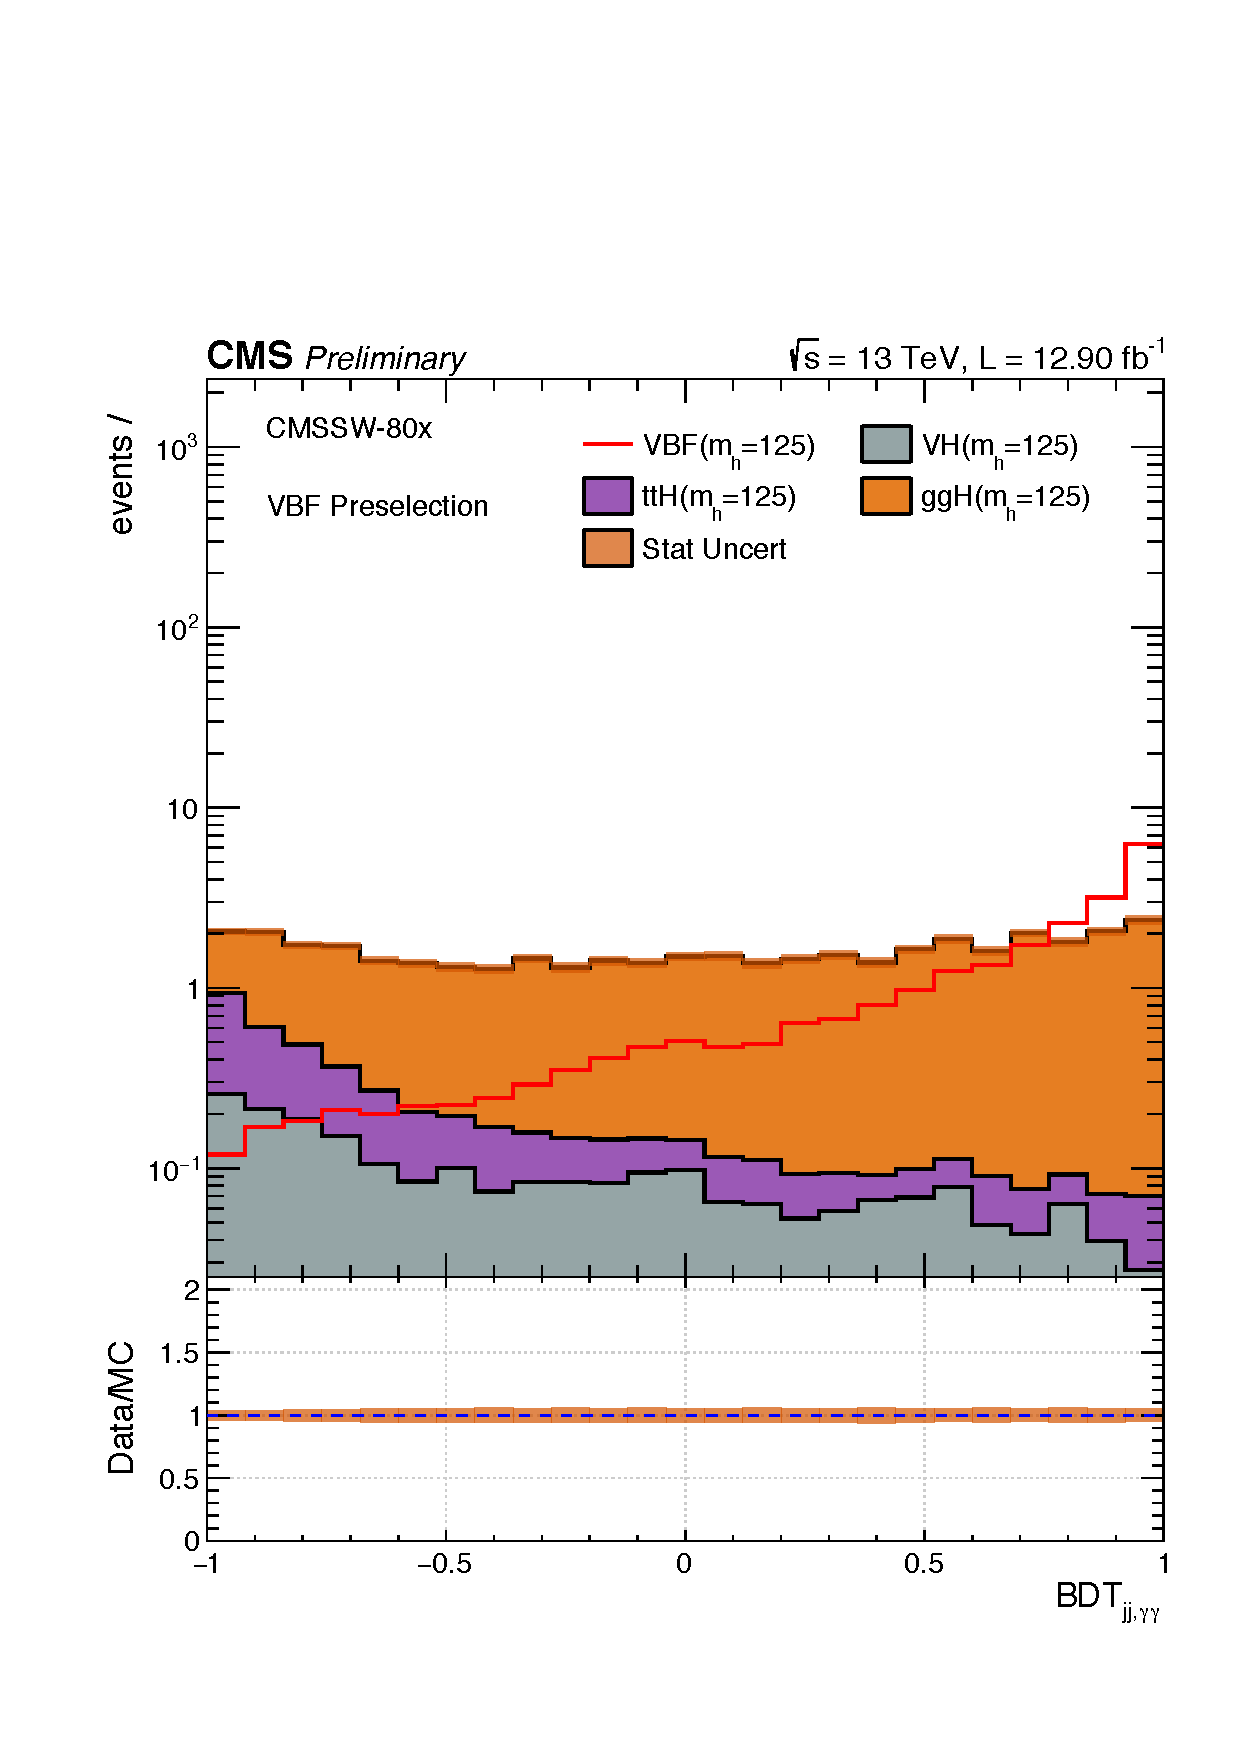
\includegraphics[width=0.45\textwidth]{catFigures/stack_histogram_dipho_dijet_MVA_signal_14-07-2016_.pdf}
\label{fig:cat:diphodijetbdt_sig}
}
 \subfloat[\DiPhoDiJetBdt output comparing data and simulated signal and background]{
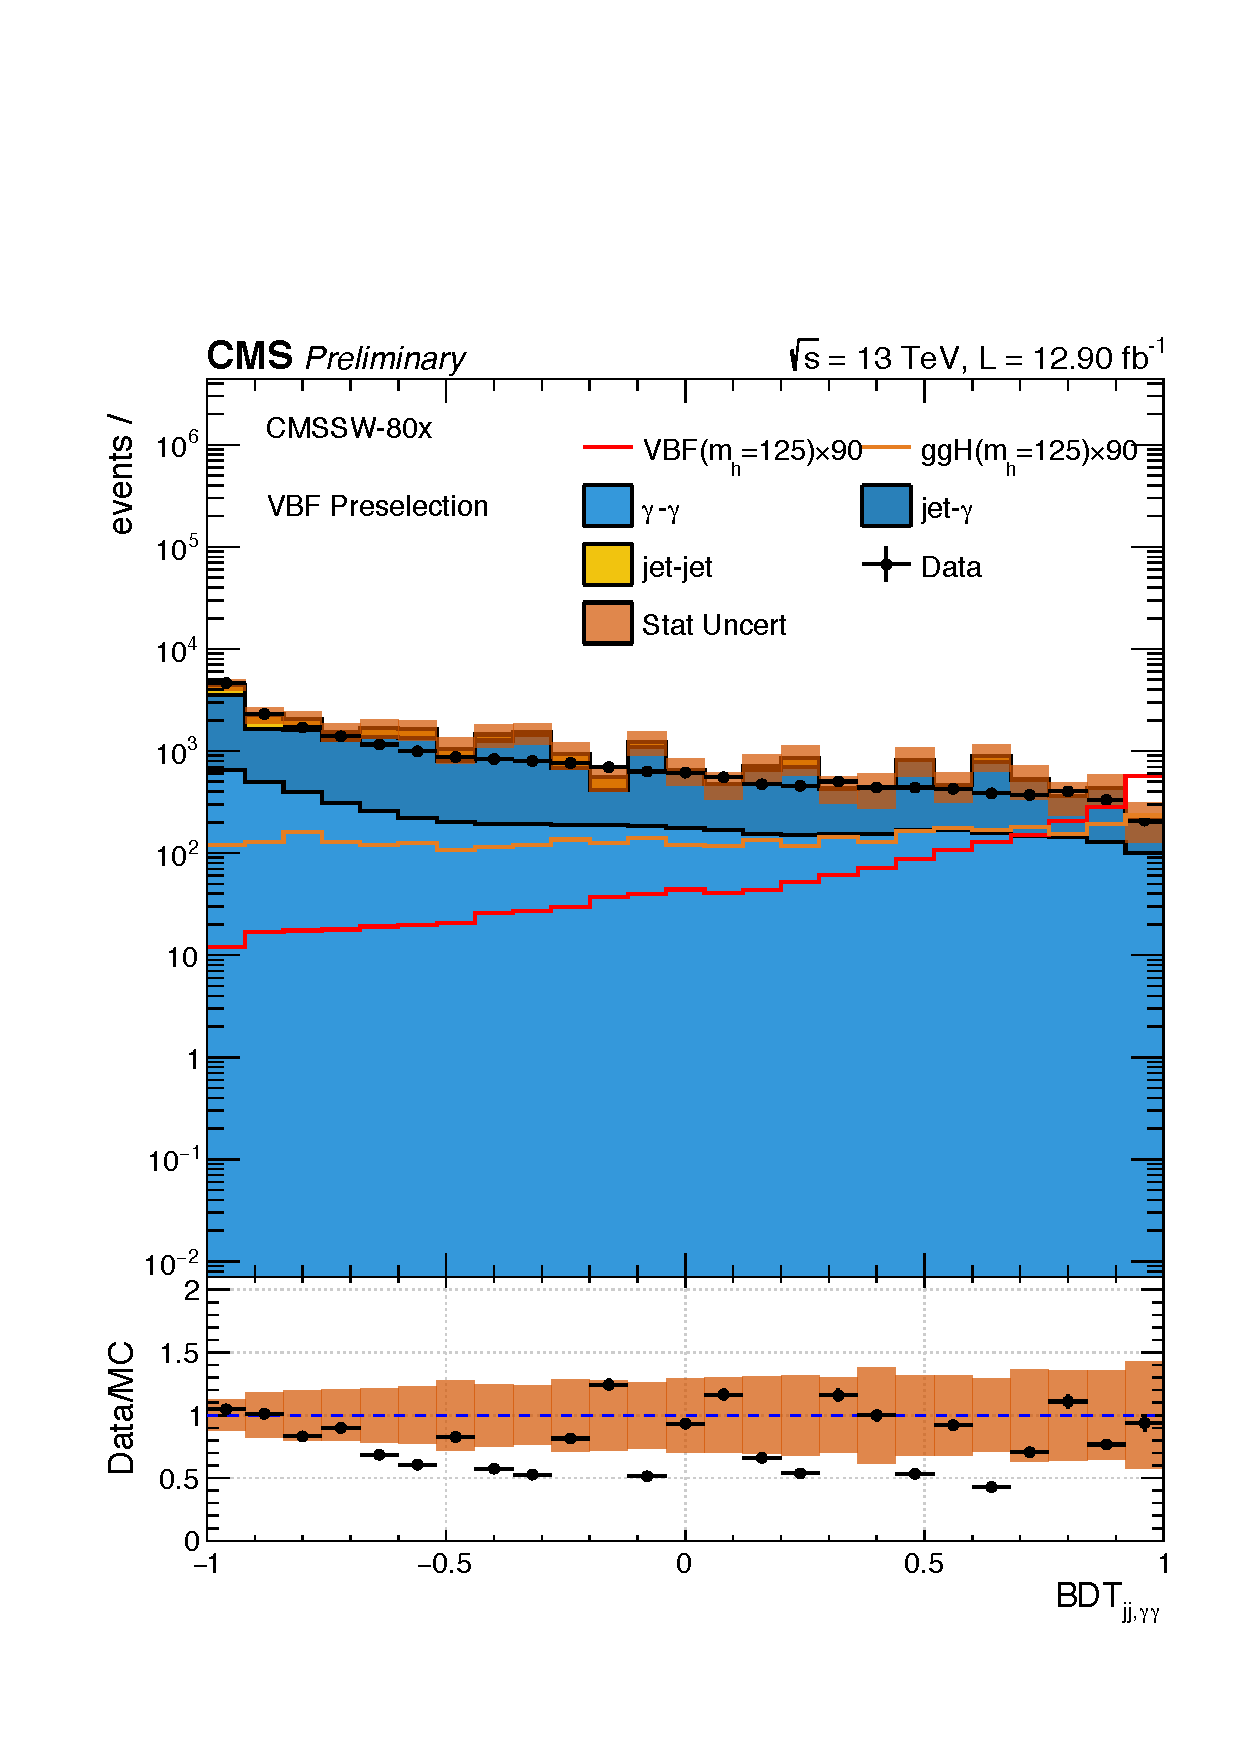
\includegraphics[width=0.45\textwidth]{catFigures/stack_histogram_dipho_dijet_MVA_VBF_14-07-2016_.pdf}
\label{fig:cat:diphodijetbdt_all}
}
\caption{The output scores of the \DiJetBdt and \DiPhoDiJetBdt split by simulated production mode and comparing data and simulated signal and background.}
\label{fig:cat:vbf_bdts}
\end{figure}

Selections on the \DiPhoDiJetBdt output score are used to define two \VBFTag categories. The most sensitive is referred to as the \VBFTag 0 category and contains all the events with the highest \DiPhoDiJetBdt output score above some boundary. The less-sensitive \VBFTag 1 category contains all events for which the \DiPhoDiJetBdt output score is below the first boundary, but still above a second boundary. Events for which the \DiPhoDiJetBdt output score is below the second boundary fail the \VBFTag categorisation, but may still be considered for inclusion in other analysis categories. %, such as the Untagged categories described in \Sec~\ref{cat:sec:untagged}. 
The location of the two boundaries is optimised first by maximising the value of the signal-to-background ratio in the \VBFTag 0 category, and then repeating the procedure after fixing the first boundary to maximise the signal-to-background ratio in the \VBFTag 1 category. Of the simulated signal events which are categorised as \VBF-like, the \VBFTag 0 category contains approximately 72\% \VBF events and 27\% \ggH events, and the \VBFTag 1 category contains approximately 55\% \VBF events and 43\% \ggH events. 


\section{\VHTag categories}
\label{cat:sec:vhtag}

\emph{\textbf{README this section will be updated with the final selections once the tags are finalised by Michael. This section uses the information from the legacy analysis as a placeholder.}}

Higgs boson events resulting from \VH production can be selected using the decay products of the $\PW$ or $\PZ$ vector boson. There several final states which can arise from these decays. First, the vector bosons can decay leptonically via $\PW \rightarrow \Plepton \Pneutrino$ or $\PZ \rightarrow \Plepton^{+} \Plepton^{-}$. Second, the vector bosons can decay to quarks which hadronize to form jets. Finally, the $\PZ$ can decay to a pair of neutrinos, which are reconstructed as a large amount of missing energy. In this analysis, the \VHLeptonicTag, \VHHadronicTag and \VHMETTag categories are respectively defined to target the final states listed above. Although the addition of the \VHTag categories does not significantly improve the overall sensitivity of the analysis, it allows the measurement of the cross-section of the \VH production mode. 

For all \VHTag categories, events must mass the preselection defined in \Sec~\ref{reco:sec:pho:preselection}. To account for the fact that the \pT spectrum of Higgs decay particles is shifted towards higher values for \VH events than for \ggH events (due to recoil against the vector boson), the leading photon \pT requirement is increased to $\pT/\mgg >1/2$ .

The \VHLeptonicTag categories target events with at least one charged lepton, and are further split into \VHLooseLeptonicTag and \VHTightLeptonicTag categories in order to maximise the sensitivity. In both cases, fewer than three jets with $\pT>20\GeV$, $|\eta|<2.4$ or within $\Delta R <0.5$ of the photons or leptons must be reconstructed in the event, to avoid selecting events from the \ttH process. The \VHTightLeptonicTag category targets the most sensitive events, i.e.~those with a fully reconstructed final state (from $\PZ$ decay) or large \MET. Events which enter this category must satisfy the following requirements:
\begin{itemize}
\item the event must contain either: one reconstructed lepton with $\pT>20\GeV$ and $\MET > 35\GeV$, or two opposite-signed same-flavour leptons both with $\pT>10\GeV$ and invariant mass in the range $[70,110]\GeV$;
\item the diphoton must pass a loose requirement on its \DiPhoBdt output score, which keeps X\% of the signal while rejecting Y\% of the background events.
\end{itemize}

Events falling in the \VHLooseLeptonicTag category must satisfy a less stringent requirement on the amount of \MET, but in this case additional selections must be added to suppress the \SM background:
\begin{itemize}
\item the event must contain exactly one reconstructed lepton with $\pT>20\GeV$ and have $\MET < 35\GeV$;
\item the invariant mass of both possible electron-photon systems must be more than 10\GeV away from the mass of the $\PZ$ boson. This is designed to reduce the contribution of $\PZ\gamma$ events, where \Zee and one of the electrons is misreconstructed as a photon; 
\item each photon in the diphoton must be separated from any reconstructed tracks by $\Delta R >1.0$ to reduce the contribution from \DY events where an electron is also misreconstructed as a photon;
\item the diphoton must pass a loose requirement on its \DiPhoBdt output score, which keeps X\% of the signal while rejecting Y\% of the background events.
\end{itemize}

The \VHMETTag category targets events where the $\PZ$ decays to two neutrinos, and thus leaves no energy in the detector. This results in a large amount of reconstructed \MET in addition to the high-\pT photons from the Higgs boson decay. Events selected by the \VHMETTag category must satisfy the following requirements, in addition to the same restriction on the number of jets as imposed on the \VHLeptonicTag categories:
\begin{itemize}
\item the event must contain $\MET > 70\GeV$;
\item the \MET direction and the momentum of the diphoton system must be separated in the $\phi$-direction by at least 2.1, since they are expected to be back-to-back due to momentum conservation;
\item the diphoton must pass a loose requirement on its \DiPhoBdt output score, which keeps X\% of the signal while rejecting Y\% of the background events.
%\item the direction of the jet with the highest \pT must be separated from the diphoton direction in the $\phi$-direction by at no more than 2.7 due to an observed correlation between t
\end{itemize}

Finally, the \VHHadronicTag category targets events where the vector boson decays to quarks, leading to two jets in the event. 
The following selections are used for this category:
\begin{itemize}
\item the leading (subleading) photon must satisfy $\pT/\mgg > 1/2$ ($\pT > 25\GeV$);
\item the event must contain at least two jets with $\pT>30\GeV$ and $|\eta|<2.4$;
\item the invariant mass of the dijet system must be in the range $[60,120]\GeV$;
\item the invariant-mass-scaled momentum of the diphoton system must be greater than $130\mgg/120$;
\item the angle $\theta^{*}$ between the diphoton direction in the diphoton-dijet rest frame and the detector frame must satisfy $|\cos{\theta^{*}}| <0.5$ to exploit differences in the angular correlation of the diphoton and the dijet for \VH events.
\end{itemize}

Events which fail the selections for the \VHTag categories may still be selected for other categories.

\section{\TTHTag categories}
\label{cat:sec:tthtag}

Higgs boson events are produced in association with a pair of top quarks in the \ttH mode. The final state therefore contains two photons from the Higgs boson decay, as well as two $\Pbottom$ quarks and decay products from two $\PW$ bosons. The $\PW$ bosons will decay either hadronically (to quarks, which subsequently hadronize to form jets) or leptonically (to a lepton and corresponding neutrino). The distinctive topologies of these events can be used to identify Higgs boson events likely to have been produced by the \ttH mechanism. The cross-section of \ttH production is low, so the benefit to the analysis in terms of final significance of an observation is small. However, the categorisation of \ttH-like events is important because it allows the measurement of the strength of the interaction of the Higgs boson with top quarks. Various extensions to the \SM predict enhanced values of the strength of the \ttH interaction, and such models can be tested through the experimental measurement of the cross-section of \ttH events decaying to \Hgg.

Two exclusive \TTHTag categories are defined in this analysis. On the one hand, the \TTHLeptonicTag category aims to select \ttH events where at least one of the $\PW$ bosons decayed leptonically. On the other hand, the \TTHHadronicTag category targets events where both $\PW$ bosons decayed to quarks. In addition to the usual preselection applied to candidate events, the requirement on the leading photon \pT is increased to $\pT>\mgg/2$, for the same reason as described in \Sec~\ref{cat:sec:tthtag}. %The selections for each of these categories are defined separately and are described below.

The leptons which are used to choose events for the \TTHLeptonicTag category must satisfy certain requirements to be used for selection purposes. Muons are required to be within $|\eta|<2.4$, pass a selection based on the properties of their tracks in the tracker and muon chambers and satisfy requirements on their \PU-corrected isolations. Electrons must pass loose identification requirements and the invariant mass of both possible electron-photon systems must be more than 10\GeV away from the mass of the $\PZ$ boson. In order to be included in the \TTHLeptonicTag category, events must satisfy the following conditions:
\begin{itemize}
\item the diphoton must satisfy a loose selection on the \DiPhoBdt output which has approximately 70\% signal selection efficiency and 15\% background selection efficiency; 
\item the event must contain at least one selected lepton with $\pT>20\GeV$; %If the lepton is an electron,n;%$Muons are required to be within $|\eta|<2.4$, pass a selection based on the properties of the tracks it leaves in the tracker and muon chambers and satisfy a requirement on its \PU-corrected charged hadron, neutral hadron and photon isolations (with cone size $R=0.4$). Electrons are required to be within the \ECAL
\item the event must contain at least 2 jets with $\pT>25\GeV$, $|\eta|<2.4$ and separated by at least a distance $\Delta R=0.4$ from a photon or lepton candidate;
\item at least one of the jets should be tagged as a $\Pbottom$ jet using the CVSv2 algorithm medium requirement, as described in~\cite{bjets}.
\end{itemize}

For events to be included in the \TTHHadronicTag category, the following selections are made:
\begin{itemize}
\item the diphoton must satisfy a loose selection on the \DiPhoBdt output score which has approximately 95\% signal selection efficiency and 45\% background selection efficiency; 
\item there must be no leptons in the event which meet the requirements for the \TTHLeptonicTag category;
\item there must be at least five jets in the event satisfying $\pT >25\GeV$;
\item at least one of the jets should be tagged as a $\Pbottom$ jet using the CVSv2 algorithm medium requirement, as described in~\cite{bjets}.
\end{itemize}

Events which fail the selections for the \TTHTag\s may still be selected for other categories.

\section{\Untagged categories}
\label{cat:sec:untagged}

Diphotons which are not categorised into the \VBF-tagged, \VH-tagged or \ttH-tagged categories can still be included in the so-called \Untagged categories, which are split into subcategories to improve the overall sensitivity of the analysis. The splitting is performed by defining boundaries in the \DiPhoBdt output score distribution. The location of the boundaries as well as the number of subcategories is optimised using simulated signal and background samples which are independent from those used to train the \DiPhoBdt. Since \ggH events are produced with only a Higgs boson in the final state to first order, they are typically placed in the \Untagged categories

The optimisation of the location of the boundaries is performed as follows. For a given number of subcategories $N_\text{subcat}$, the boundaries are initially spaced evenly throughout the \DiPhoBdt output score distribution. Events falling in the subcategory below the lowest boundary are discarded. Simplified models are used to parametrise the signal and background \mgg distributions in the remaining categories. For the signal, the model is a sum of two Gaussian functions, which model the detector resolution and the uncertainty due to incorrect vertex assignment respectively. For the background, the \mgg spectrum is modelled using an exponential shape. The expected significance is then obtained by producing an Asimov dataset~\cite{Cowan:2010js} from the signal and background models in each category, and then performing a simultaneous signal and background fit. The estimation of the expected significance is iteratively repeated, allowing the boundaries between the subcategories to float. The final set of boundaries is chosen such that the expected significance is maximised for a given $N_\text{subcat}$.

The procedure can be repeated separately for arbitrary values of $N_\text{subcat}$. In this analysis, $N_\text{subcat}=4$ (ignoring the subcategory below the lowest boundary) was chosen, as moving to $N_\text{subcat}=5$ produced a negligible improvement in the expected significance. The boundaries extracted from this optimisation procedure are represented by the vertical dashed lines in \Fig\s~\ref{fig:cat:diphobdt_a} and~\ref{fig:cat:diphobdt_b}. The resulting \Untagged categories are numbered from Untagged 0 (most sensitive) to \Untagged 3 (least sensitive), and events where the diphoton has a \DiPhoBdt score too low to enter \Untagged 3 are discarded.

\section{Categorisation hierarchy}
\label{cat:sec:hierarchy}
Each event can be assigned to only one category. To ensure this, a categorisation hierarchy is enforced. Each event is tested to see if it can be included in the first category in the hierarchy. If it satisfies the relevant requirements, the event enters the category and the categorisation is done. If not, the next category in the hierarchy is tested, and so on. If no further categories remain, the event is discarded. The hierarchy is as follows, with categories ordered from first tested to last tested: \TTHLeptonicTag, \VHTightLeptonicTag, \VHLooseLeptonicTag, \VHMETTag, \TTHHadronicTag, \VHHadronicTag, \VBFTag 0, \VBFTag 1, \Untagged 0, \Untagged 1, \Untagged 2, \Untagged 3.


